%!TEX root = ../Thesis.tex
\chapter{Introduction}\label{cha:introduction}
%
% This introductory chapter will briefly provide context for the material/results presented in this report and give motivation and a description of the problem to be solved. A literature review summarizes existing relevant knowledge, and establishes the foundation of the later control system. The scope of the work is then defined through a list of assumptions. Finally, the contributions of the thesis are defined and elaborated.

This is a master thesis written in cooperation between NTNU and Hymatek Controls. Hymatek Controls is a company located in Oslo, that delivers equipment and control systems to hydro electric power plants world wide. The company is now extending its portfolio with condition monitoring. Hymatek has acquired a large dataset containing data from a five year period for $27$ hydro electric power-plants. The goal of this thesis is to find possible use cases for condition monitoring in the provided dataset, research possible techniques and implement some of them on the found use case. Since this is a new research area for Hymatek, this thesis will cover a wide range of aspects. 

This chapter provides an introduction to the work done, describing the motivation and problem description for the thesis. In addition a literature review looking into state of the art techniques used for condition monitoring. 


\section{Motivation}\label{sec:motivation}

% % What is the motivation for considering the problems/question that you approach in your work? Why is this an interesting problem? The motivation should instead describe why it is interesting from a societal point of view, and/or from a scientific point of view.

The need for renewable and stable energy sources is great in both Norway, Europe and world wide. According to \cite{Statkraft2009} $99\%$ of the Norwegian power production comes from hydro electric power plants. Almost $50\%$ of Europe's hydro electric capacity is located in Norway. Hydro electric power is seen as one of the most stable and cleanest energy sources one can find \cite{Statkraft2009}. As many European countries are transitioning into renewable energy sources, the need for stable and controllable power sources grows. Both wind and solar power production is dependent on weather conditions, and their production capacity can change quickly and unexpectedly. Norway has been called Europe's renewable battery due to its hydro electric capacity, and the capacity to deliver power is growing. By 2121 Norway and Great Britain will be connected through a new underwater power cable. This is an example that shows that Norway is becoming a part of a more complex energy market. As the exporting capacity grows, green energy from Norway can be supplied to reduce the consumption of fossil energy from for example coal from the European continent. This means that increased productivity and efficiency in hydro electric power plants, effectively can reduce the carbon footprint of the European power production. 

One way to increase a plant's productivity is to ensure that it is in an operable state at all times. This is however not possible, since one has to perform maintenance on all parts of a plant. But planned maintenance is not the only reason for a power plant stopping down. Components can breakdown outside of their service interval, and this can lead to unplanned downtime. This is of course not only a case for hydro electric power plants, but for more or less any industry or factory. Unplanned downtime is expensive for the energy company that operates the plant, and depending on the time of year and the duration of the breakdown the cost can have a large impact on their operation. Finding a way to avoid these breakdowns, and replacing unplanned maintenance with planned maintenance is something all energy companies are interested in. A hydro electric power plant contains several large components such as turbines, transformers, hydraulic systems, valves, pipes etc. In addition you have all the equipment needed to operate the system. Keeping spare parts for all components would require an enormous storage, in addition to tie large assets due to the cost of all components. In addition many components don't need to be replaced often, hence the spare can be left in storage for many years. Clearly this is not a very good solution. 

Another approach is to try to eradicate unexpected breakdowns. This means that one need to have a way to detect that a component is decaying, so that one can plan an overhaul or replacement before it breaks down. This also solves another factor to consider when it comes to breakdowns  of components, the domino effect. Depending on the situation and the component, if one component breaks down, it might end up taking several other with it. If a bearing on a turbine shaft breaks down, one risks that the damage will spread to the bearing on the other side of the shaft, and even to the turbine it self. A continuous analysis of the condition of the bearing could help avoid this issue. This is known as condition monitoring. In its most complete form, condition monitoring gives an insight into the condition of the monitored components, giving an estimate to the remaining lifetime of the component. Introducing condition monitoring could help reduce the number of breakdowns, as components can be replaced before breaking. \todo{add citation?}

There are many good reasons for pursuing the topic of this thesis, on a personal level it is motivating to work with real world data, to learn the difference between theoretical and practical engineering. Looking for solutions that will improve the operation of a hydro electric power plant, which can give even more clean energy is also motivating. Additionally, the fact that possible solutions found for the specific cases looked into most likely can be adapted to other industries is also very motivating. 

An attempt of classifying the wear of the guide vanes on a Francis turbine were performed in my project thesis.  


This triggered my interest for the possibilities of information found in data. 
% Looking into different possible techniques for condition monitoring that can be utilized on a real world dataset will give
% As the world become more and more digitized, one can either keep up, or be left behind. Condition monitoring is seen as an important part of the future portfolio of Hymatek Controls, and a necessary addition to continue their growth into the future. 


\section{Problem definition}

% Korleis oppsto problemstillinga? dreiv å såg gjennom feiloggen etter interesssante feil. Såg då at det var problemer med nålstryinga for hjartdøla. Starta så å undersøke dataen, og fant etterkvart ut at det er 2 anlegg til som har nålstyring. Dei hadde derimot ikkje raportet feil med nålene, noko som gav meg grunn til å tenke at dei har normal oppførsel. Då kunne eg og starte å samanlikne data mellom kraftverka for å sjå kva som er unormal og normal oppførsel.

No exact problem definition were provided by Hymatek, they provided a dataset containing process-data from $27$ hydro electric power plants for the period $2014-2017$, and gave no restriction on which plants and cases that could be investigated. A historical incident log were also provided for all plants, with varying level of detail. Based on this, the problem definition was split into three main parts. As this is a thesis built upon an unknown dataset with unknown quality, an important factor is to recognize what the data can be utilized for, and what improvements that could/needs to be done to make the data analysis more extensive. Ideally the result of the thesis will be a system for condition monitoring for a real world case found in the dataset. However, since Hymatek is still in the start up phase of its condition monitoring research, all experiences from this thesis are valuable. Therefore the most important part of the thesis is to understand why or why not one is able to create a condition monitoring system for the given case. Then this thesis can be used as a basis for further condition monitoring case analysis. The three parts are as follows: 

\begin{itemize}
    \item Data acquisition and case extraction. The provided data is not ready for analysis, one needs to extract datasets for each of the plants. Once the data is on a format that can be analyzed, the historical data from the plants and the datasets needs to be analyzed to build a  case for the further analysis. 
    \item Finding techniques suitable for condition monitoring for the case found.  
    \item Analyzing the case using the techniques found. Emphasize on how the different techniques perform, and what can/needs to be done to improve the performance. 
\end{itemize}


% \section{Literature review}\label{sec:review}
    

% Start writing about the articles I have already read, can always delete it if it is not relevant in the end. 
%     \subsection{Timeseries forecasting}\label{sec:time_series_forecasting}
    
%     \subsection{One class support vector machine novelty/anomaly detection}\label{sec:ocsvm_novelty_detection}
    
%     \subsection{Neural network novelty/anomaly detection}\label{sec:nn_novelty_detection}
    
%     \subsection{The data set}\label{sec:the_data}
%     The data is provided by Hymatek controls, and is collected from more than 30 hydro electric power plants around Norway, in the period between $01.01.2014$ and $01.07.2017$. 

\section{Assumptions}\label{sec:assumptions}
    Since the thesis span over many different research areas, only one case will be analyzed, even if it should be possible to find several more from such an extensive dataset. In addition only a subset of the suggested techniques will be chosen for anlysis, spanning from easy to more complex. There might be algorithms not tested that could be useful for the given case. The techniques are chosen in cooperation with Hymatek. 
    
    Availability of computing power and memory also introduces constraints to the analysis. All analysis are performed on a desktop from dell provided by NTNU. This means that no analysis will be performed using the full datasets, they will be reduced by either feature selection or dimensionality reduction. 
    
    Condition monitoring is a wide field, and creating a full scale codition monitoring system for one case is to comprehensive. The thesis will therfore foucs on anomaly/novelty detection for the given case. This means that one will train different techniques on normal operation data, and verify how well the different techniques are able to detect the anomaly found for the specific case. 
    
\section{Hydro electric power production}\label{ref:sec_hydropower}
    \todo{Add more information? explaing francis aswell?}
    $99\%$ of the Norwegian power production comes from hydro electric power plants. Hydro electric power is clean, reliable and once built, it produces cheap energy. \cite{Statkraft2009} claims that no other types of power plants has longer expected life time and higher efficiency than hydro electric power. Statkraft also states that countries with the highest increase in energy demand is also countries with the highest unused potential for hydro electric power. This means that hydro electric power production can play a big role in the hunt for meeting a global power demand. There are many old power plants today, so there is also possibilities for modernization and extensions of already existing plants. 
    
    The principal behind hydro electric power is simple. It utilizes the energy in running water and the energy is converted using a turbine. There two main types of turbines, impulse and reaction \cite{Paish2002}. The difference between the two types is found in how the rotational force is created. The impulse turbine rotor runs in air, and rotational force is created by a water jet lead onto the turbine blades. The reaction turbine is submerged in water, and the rotational force comes from a lift force created by the oncoming water flow. For the impulse turbine only kinetic energy is used to generate the rotational force, for the reaction both kinetic and pressure energy is used. When the water hits the turbine blades the water pressure is reduced to atmospheric pressure, and all pressure energy is converted to kinetic energy. For the reaction turbine, which is submerged in water, the water pressure is still high, meaning that one need a casing which is sealed from atmospheric pressure. 
    
    \begin{figure}
        \centering
        \includegraphics{}
        \caption{Principal behind reaction and impulse turbines}
        \label{fig:my_label}
    \end{figure}
    
    
    The two most common turbine types are Francis and Pelton. The type used is mostly defined by the size of the flow and the head of the water. Whether the turbine will be producing power only at optimal flow, or if it will be used for power production over a wider range is also a criterion. 
    
    
    
    \subsection{Pelton turbines}\label{subsec:pelton}
        
        The Pelton turbine is the most common impulse turbine. Water is lead onto to the turbine through a series of needles or valves. The turbine has a set of buckets located on the turbine wheel which splits the water jet in two, where each half is deflected back and falls down into a discharge channel, \cite{Paish2002}. A cross section of a Pelton turbine is seen in figure \ref{fig:pelton_turbine}. As one can see the needles are divided equally arround the turbine. The amount of produced power is controlled by the number of active needles, and by regulating their opening. Figure \ref{fig:pelton_bucket} shows how the buckets are designed. Where the water jets hits the buckets is easily verifiable by looking at the corroded parts of the buckets. The needles are controlled by a hydraulic system, which is controlled by the power plant control system. 
        
        
        \begin{figure}
            \begin{minipage}[b]{0.5\linewidth}
                \centering
                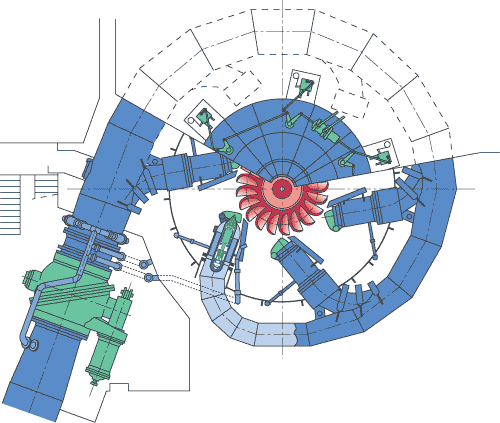
\includegraphics[width = 0.9\textwidth]{report/figures/introduction/pelton.png}
                \caption{Cross section of a Pelton turbine with $6$ needles. Courtesy of Voith Siemens Hydro Power Generation, GFDL, Wikimedia Commons.} %\url{https://commons.wikimedia.org/wiki/File:S_vs_pelton_schnitt_1_zoom.png}
                \label{fig:pelton_turbine}
            \end{minipage}
            \begin{minipage}[b]{0.5\linewidth}
                \centering
                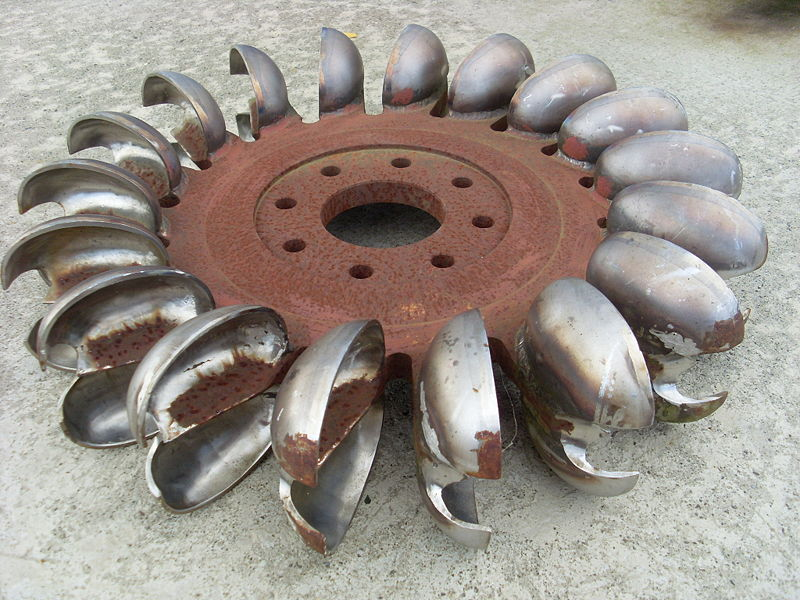
\includegraphics[width = 0.9\textwidth]{report/figures/introduction/pelton_bucket.jpg}
                \caption{A Pelton turbine wheel, the split buckets are easily visible. Courtesy of Zedh, CC-BY-SA, Wikimedia Commons. } %\url{https://commons.wikimedia.org/wiki/File:Pelton_400kW_roue_1.JPG}
                \label{fig:pelton_bucket}
            \end{minipage}
        \end{figure}
        
        
    
    \subsection{Francis turbines}\label{subsec:francis}
        The Francis turbine is a reaction turbine. The water is lead onto the turbine through a set of guide vanes connected to the spiral casing, and lead out from the centre of the turbine. The guide vanes controll the amount of water lead onto the turbine, and hence the amount of produced energy. A cross section of a Francis turbine is seen in figure \ref{fig:francis}. The guide vanes can be operated from tangential to perpendicular. All guide vanes have the same opening, and are controlled through a ring mounted on the top of the turbine. Figure \ref{fig:guide_vanes} shows a hydraulic actuator used to control the ring that operates the guide vanes. As for the pelton turbine, the hydraulics is again controlled by the plants controll system.  
        
        \begin{figure}
            \begin{minipage}[b]{0.5\linewidth}
                \centering
                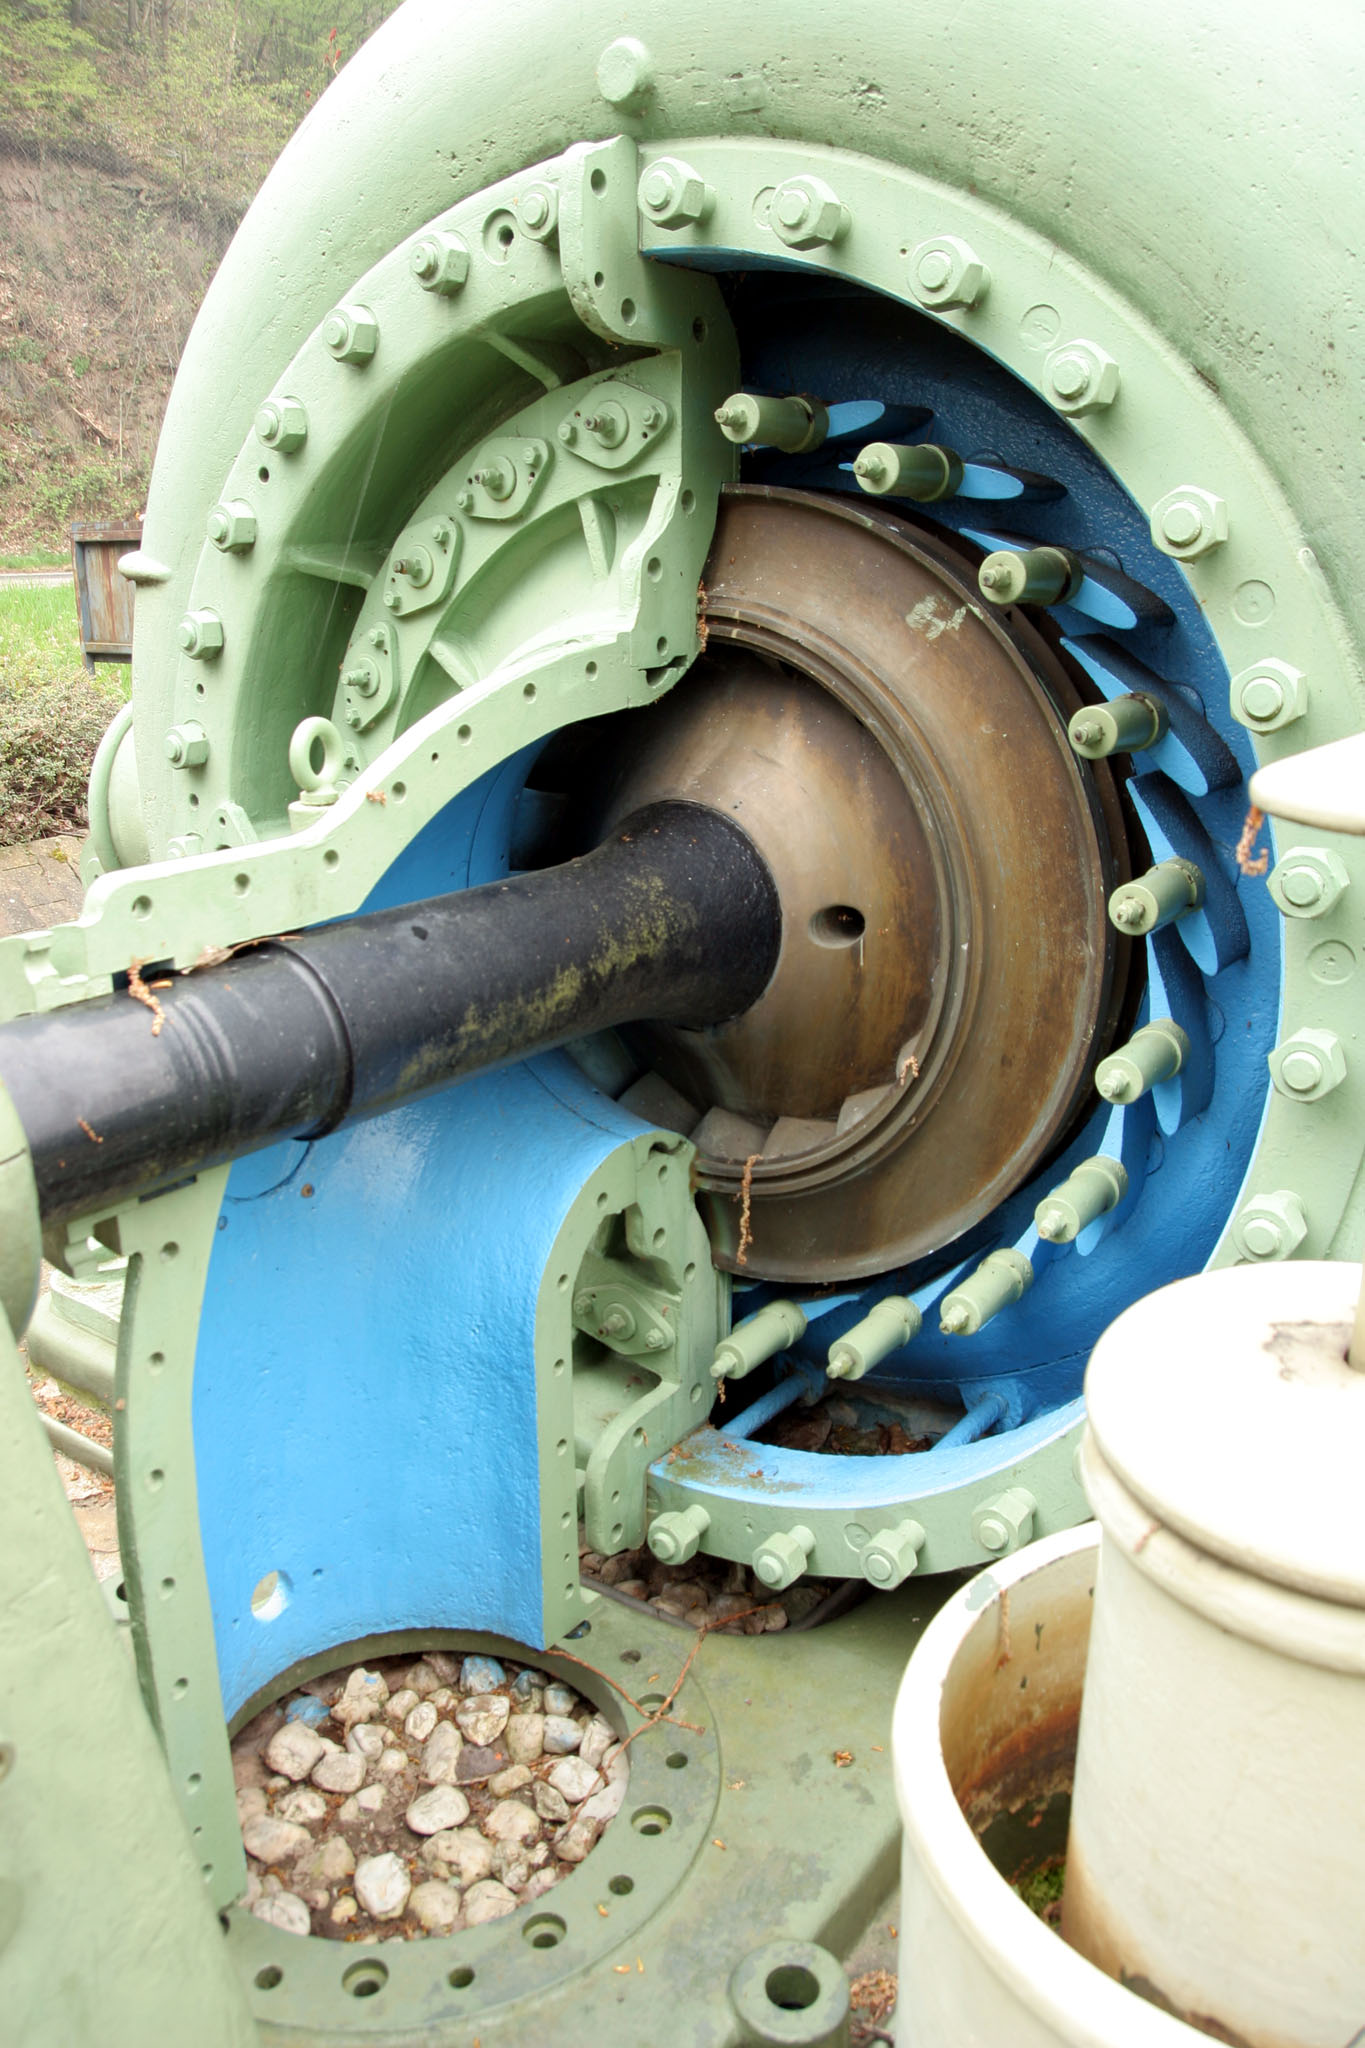
\includegraphics[width = 0.9\textwidth]{report/figures/introduction/francis_turbine.jpg}
                \caption{Cross section of a Francis turbine. Courtesy of Armin Kübelbeck, CC-BY-SA, Wikimedia Commons.} %https://commons.wikimedia.org/wiki/File:Fankel_Francisturbine_01.jpg
                \label{fig:francis}
            \end{minipage}
            \begin{minipage}[b]{0.5\linewidth}
                \centering
                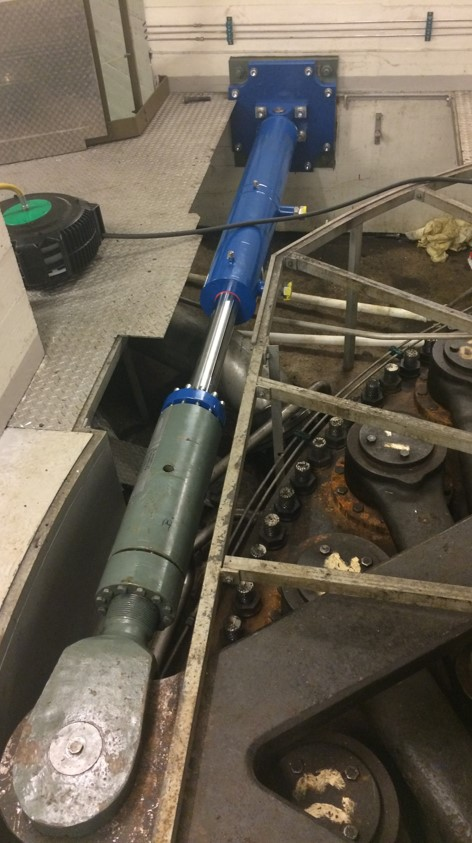
\includegraphics[width = 0.9\textwidth]{report/figures/introduction/servo1(1).jpg}
                \caption{Hydraulic actuator for guide vane controll. Courtesy Hymatek Controls}
                \label{fig:guide_vanes}
            \end{minipage}
        \end{figure}
        
    \subsection{Other equipment}
        There are several other large components in a hydro electrical power plant. Among them are;
        \begin{itemize}
            \item Generator
            \item Transformers
            \item Coolers
        \end{itemize}
        These are not explained in any further detail, because they are not a part of the case analyzed. 
% \section{Background and Contributions}\label{sec:contributions}
% Here you describe the main contributions of your project work: What are the new results - the achievements - of your work. 

% It is important that you here also clearly describe which background material you have received. Which information, software, equipment etc. have been made available for you, or form the basis for your work. Which help and support have you received, and from who, during your work. For instance: The Matlab simulator used in Section 2 was provided to me by PhD candidate NN, and I have adapted this to the problem in this thesis by modifying ....

% \section{Outline}\label{sec:outline}
% The report is organized as follows. In Chapter~\ref{cha:first} a mathematical model is developed to describe the system... In Chapter
